\begin{figure}[t]
\centering
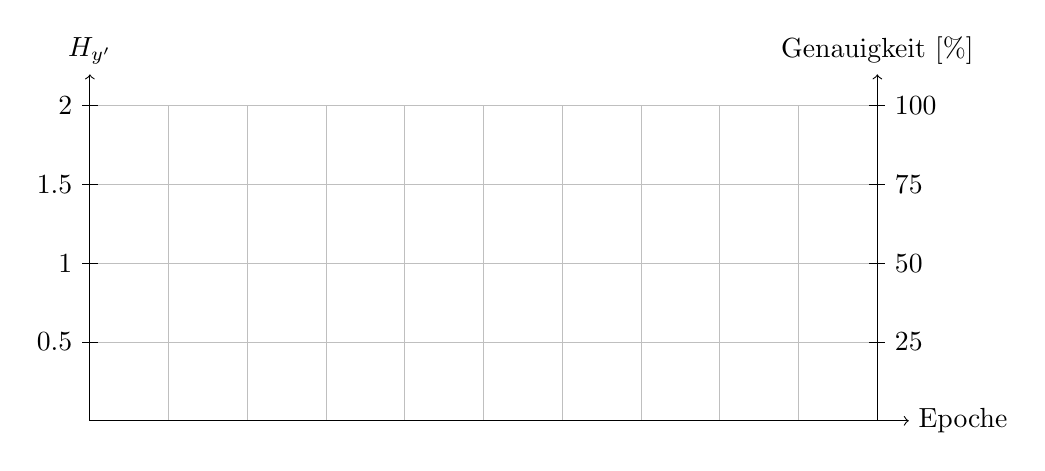
\begin{tikzpicture}
  \draw[color=lightgray] (0, 0) grid (10, 4);

  \draw[->] (0,  0) -- (10.4, 0) node[right] {Epoche};
  \draw[->] (0,  0) -- (0,  4.4) node[above] {$H_{y^{\prime}}$};
  \draw[->] (10, 0) -- (10, 4.4) node[above] {Genauigkeit [\%]};

  \draw (0.1, 4) -- (-0.1, 4) node[left] {$2$};
  \draw (0.1, 3) -- (-0.1, 3) node[left] {$1.5$};
  \draw (0.1, 2) -- (-0.1, 2) node[left] {$1$};
  \draw (0.1, 1) -- (-0.1, 1) node[left] {$0.5$};

  \draw (9.9, 4) -- (10.1, 4) node[right] {$100$};
  \draw (9.9, 3) -- (10.1, 3) node[right] {$75$};
  \draw (9.9, 2) -- (10.1, 2) node[right] {$50$};
  \draw (9.9, 1) -- (10.1, 1) node[right] {$25$};

\end{tikzpicture}
  \caption[\gls{Cifar}-10 Training]{}
\label{fig:cifar_10_train}
\end{figure}
